\section{What is SQL?}
\begin{itemize}
    \item SQL is a language used to interact with relational database management systems.
    \item A relational database management system is basically just a software application to create and manage different databases.
\end{itemize}


%----------------------------------------------------------------------------------------
\section{What is a database?}
\begin{itemize}
    \item Sometimes databases are abbreviated as DB.
    \item A database is any collection of related information:
        \begin{itemize}
            \item Phone book.
            \item Shoping list.
            \item Todo list.
            \item Your 5 best friends.
            \item Facebook's User base.
        \end{itemize}
    
    \item Database can be stored in different ways.
        \begin{itemize}
            \item On paper.
            \item In your mind.
            \item On a computer.
            \item This PowerPoint.
            \item Comments section.
        \end{itemize}
\end{itemize}

\section{Computers with databases}
\begin{itemize}
    \item Storing a collection of related information on a computer is extremely useful, computers are great for this.
    \item A database can be stored anywhere, but there are better ways of storing databases than others. Computers are great at keeping track of large amounts of information.
    \item Take this example:
        \begin{center}
            \begin{tabular}{ |p{7cm}|p{7cm}| }
                \hline
                    Amazon.com & Shopping list \\
                \hline
                    {\begin{itemize}
                        \item Keeps track of products, reviews, purchase orders, credit cards, users, media, etc.
                        \item Needs to store trillions of pieces of information, and they need to be readily available.
                        \item Information is extremely valuable and critical to Amazon.com's functioning.
                        \item Security is essential, Amazon stores peoples' personal information:
                            \begin{itemize}
                                \item Credit card \#, SSN, Address phone.
                            \end{itemize}
                        \item Information is stored on a computer.
                    \end{itemize}}
                    & 
                    {\begin{itemize}
                        \item Keeps track of customer products that need to be purchased.
                        \item Stores 10-20 pieces of information, this also needs to be readily available.
                        \item Information is for convenience sake only and not necessary for shopping.
                        \item Security is not important.
                        \item Information is stored on a piece of paper, or even just in someone's memory.
                    \end{itemize}}
                    \\ 
                \hline
            \end{tabular}
        \end{center}
\end{itemize}

\section{Database Management System (DBMS)}
\begin{itemize}
    \item A database can be as simple as a txt file, or excel file, but generally if you need to store large amounts of information a better solution is to use special software designed to create and maintain a database, this is called a Data Management System.
    \item A special software program that helps users create and maintain a database.
        \begin{itemize}
            \item Makes it easy to manage large amounts of information.
            \item Handles security.
            \item Backup your data.
            \item Importing and exporting data.
            \item Concurrency.
            \item Interacts with software applications:
                \begin{itemize}
                    \item Programming software.
                \end{itemize}
        \end{itemize}
    
    \item The database management system is not the database it is the software application that is creating, managing, updating, etc the database.
        \begin{figure}[H]
            \centering
            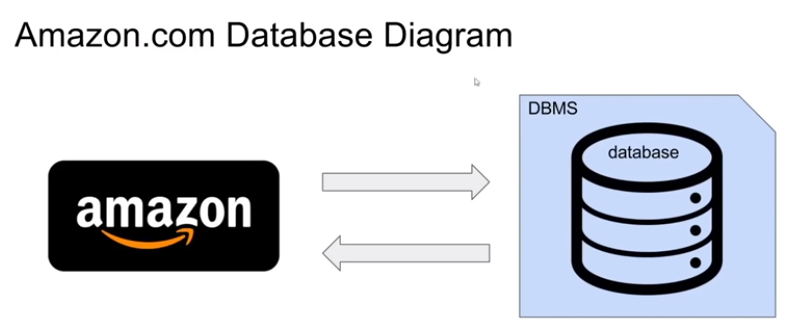
\includegraphics[width=0.4\textwidth]{./figs/dbamazon.png}
        \end{figure}
\end{itemize}

\section{C.R.U.D}
\begin{itemize}
    \item Create, Read (Retrieve), Update, Delete.
    \item CRUD represents the 4 main operations that can be done in a database.
    \item Any good database management systems are able to perform these operations.
\end{itemize}

\section{Two types of databases}
\begin{itemize}
    \item Relational Database (SQL): (The most popular kind of database.)
        \begin{itemize}
            \item Organize data into one or more tables.
            \item Each table has columns and rows.
            \item A unique key identifies each row.
            \item It is a lot like an Excel spreadsheet.
        \end{itemize}
    
    \item Non-relational (noSQL / no just SQL):
        \begin{itemize}
            \item Organize data is anything but a traditional table.
            \item Key-value stores.
            \item Documents (JSON, XML, etc).
            \item Graphs.
            \item Flexible tables.
            \item Any type of database that is not a non-relational database. Organize data in anything but a table.
        \end{itemize}
\end{itemize}

\section{Relational Database (SQL)}
\begin{figure}[H]
    \centering
    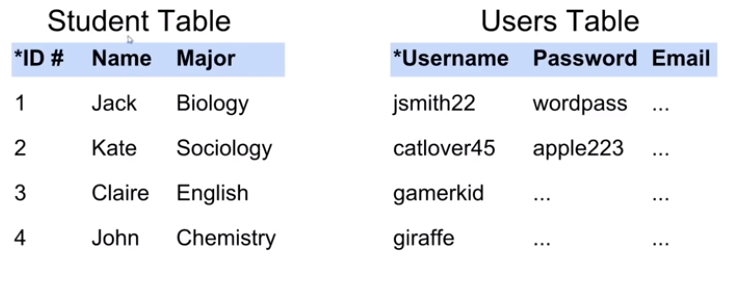
\includegraphics[width=0.4\textwidth]{./figs/relational.png}
\end{figure}
\begin{itemize}
    \item Relational Database Management Systems (RDBMS):
        \begin{itemize}
            \item Help users create and maintain a relational database.
                \begin{itemize}
                    \item mySQL, Oracle, postgreSQL, mariaDB, etc. 
                \end{itemize}
        \end{itemize}
    
    \item Structured Query Language (SQL):
        \begin{itemize}
            \item Relational Database Systems use SQL to interact with relational DB.
            \item Used to perform CRUD operations, as well as other administrative tasks (user management, security, backups, etc.)
            \item Used to define tables and structures.
            \item SQL code used on one RDBMS is not always portable to another without modification. Not all SQL code used on one RDBMS will be able to be used on others.
        \end{itemize}
\end{itemize}

\section{Non-relational databases}
\begin{itemize}
    \item Anything that is not relational.
    \item For example: 
        \begin{figure}[H]
            \centering
            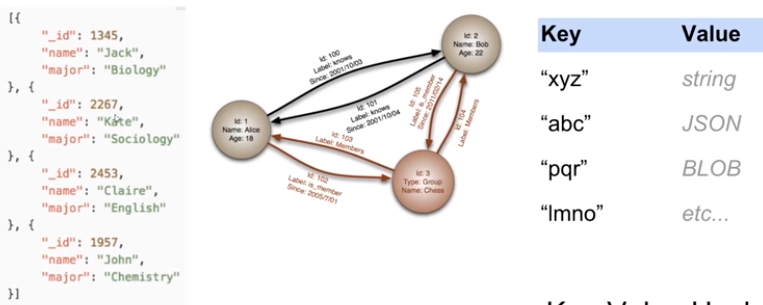
\includegraphics[width=0.4\textwidth]{./figs/nonrelational.png}
        % 	\caption{\href{}{source}}
        \end{figure}
        \begin{itemize}
            \item Store data on graphs, nodes, key value hash, documents (JSON, BLOB, XML).
        \end{itemize}
    
    \item Non-relational Database management systems (NRDBMS):
        \begin{itemize}
            \item Help users create and maintain a non-relational database.
                \begin{itemize}
                    \item mongoDB, dynamoDB, apache cassandra, firebase, etc.
                \end{itemize}
            
            \item Implementation specific:
                \begin{itemize}
                    \item Unlike RDMBS where there is a standard (SQL), this is implementation specific, there is no standard language for interacting with the non-relational database. 
                    \item Each implementation will include the implementation for managing the database and performing the CRUD operations.
                    \item Most NRDBMS will implement their own language for performing CRUD operations and administrative operations on the database.
                \end{itemize}
        \end{itemize}
\end{itemize}

\section{Database Queries}
\begin{itemize}
    \item Queries are request made to the database management system for specific information:
        \begin{itemize}
            \item Query is asking the DBMS for information.
        \end{itemize}
    \item As the database's structure becomes more and more complex it becomes more difficult to get the specific pieces of information we want.
    \item A Google search is a query.
        \begin{itemize}
            \item With a relational database management system we cannot search for information in the same way google searches for it, we must adhere to a specific language in this case SQL.
        \end{itemize}
\end{itemize}

\section{Wrap up}
\begin{itemize}
    \item Database is any collection of related information.
    \item Computers are great for storing databases.
    \item Database Management Systems (DBMS) make it easy to create, maintain and secure a database.
    \item DBMS allow you to perform the CRUD operations and other administrative tasks.
    \item Two types of databases, relational and non-relational.
    \item Relational databases use SQL and store data in tables with rows and columns.
    \item Non-relational databases store data using other data structures.
    \item Queries are request made to the database management system for specific information.
\end{itemize}
